\begin{figure}[ht!]
\begin{subfigure}{0.33\textwidth}
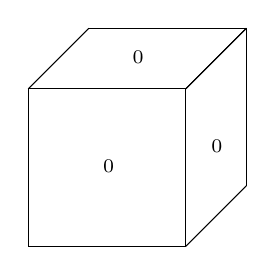
\begin{tikzpicture}[scale=0.5]
\foreach \x in{0,4}
{   \draw (0,\x ,4) -- (4,\x ,4);
    \draw (\x ,0,4) -- (\x ,4,4);
    \draw (4,\x ,4) -- (4,\x ,0);
    \draw (\x ,4,4) -- (\x ,4,0);
    \draw (4,0,\x ) -- (4,4,\x );
    \draw (0,4,\x ) -- (4,4,\x );
}
\node at (0.5,0.5) {\scriptsize $0$};
\node at (3.25,1.0) {\scriptsize $0$};
\node at (1.25,3.25) {\scriptsize $0$};
\end{tikzpicture}
\caption{Level 0}
\end{subfigure}%
\begin{subfigure}{0.33\textwidth}
\centering
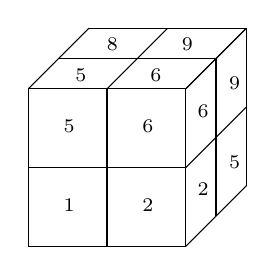
\begin{tikzpicture}[scale=0.5]
\foreach \x in{0,2,4}
{   \draw (0,\x ,4) -- (4,\x ,4);
    \draw (\x ,0,4) -- (\x ,4,4);
    \draw (4,\x ,4) -- (4,\x ,0);
    \draw (\x ,4,4) -- (\x ,4,0);
    \draw (4,0,\x ) -- (4,4,\x );
    \draw (0,4,\x ) -- (4,4,\x );
}
\node at (-0.5,-0.5) {\scriptsize $1$};
\node at (1.5,-0.5) {\scriptsize $2$};
\node at (-0.5,1.5) {\scriptsize $5$};
\node at (1.5,1.5) {\scriptsize $6$};
\node at (2.9,-0.1) {\scriptsize $2$};
\node at (3.7, 0.6) {\scriptsize $5$};
\node at (2.9, 1.9) {\scriptsize $6$};
\node at (3.7, 2.6) {\scriptsize $9$};
\node at (-0.2, 2.8) { \scriptsize $5$};
\node at (1.7, 2.8) { \scriptsize $6$};
\node at (0.6, 3.6) { \scriptsize $8$};
\node at (2.5, 3.6) { \scriptsize $9$};
\end{tikzpicture}
\caption{Level 1}
\end{subfigure}%
\begin{subfigure}{0.33\textwidth}
\centering
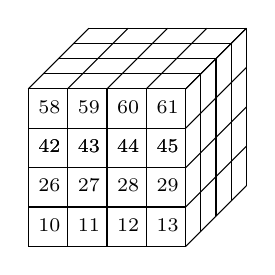
\begin{tikzpicture}[scale=0.5]
\foreach \x in{0,...,4}
{   \draw (0,\x ,4) -- (4,\x ,4);
    \draw (\x ,0,4) -- (\x ,4,4);
    \draw (4,\x ,4) -- (4,\x ,0);
    \draw (\x ,4,4) -- (\x ,4,0);
    \draw (4,0,\x ) -- (4,4,\x );
    \draw (0,4,\x ) -- (4,4,\x );
}
\node at (-1.0,-1.0) {\scriptsize $10$};
\node at ( 0.0,-1.0) {\scriptsize $11$};
\node at ( 1.0,-1.0) {\scriptsize $12$};
\node at ( 2.0,-1.0) {\scriptsize $13$};
\node at (-1.0, 0.0) {\scriptsize $26$};
\node at ( 0.0, 0.0) {\scriptsize $27$};
\node at ( 1.0, 0.0) {\scriptsize $28$};
\node at ( 2.0, 0.0) {\scriptsize $29$};
\node at (-1.0, 1.0) {\scriptsize $42$};
\node at ( 0.0, 1.0) {\scriptsize $43$};
\node at ( 1.0, 1.0) {\scriptsize $44$};
\node at ( 2.0, 1.0) {\scriptsize $45$};
\node at (-1.0, 1.0) {\scriptsize $42$};
\node at ( 0.0, 1.0) {\scriptsize $43$};
\node at ( 1.0, 1.0) {\scriptsize $44$};
\node at ( 2.0, 1.0) {\scriptsize $45$};
\node at (-1.0, 2.0) {\scriptsize $58$};
\node at ( 0.0, 2.0) {\scriptsize $59$};
\node at ( 1.0, 2.0) {\scriptsize $60$};
\node at ( 2.0, 2.0) {\scriptsize $61$};
\end{tikzpicture}
\caption{Level 2}
\end{subfigure}
\caption{Global unique identifiers: $\ID(l,i,j,k)$ for an octree}
\label{fig:tree_global_IDs}
\end{figure}
